\Chapter{Tensorflow és Keras}

A dolgozat programjának megvalósításához a TensorFlow függvénykönyvtárat választottam ki. A TensorFlow egy ingyenes, open-source gépi tanulásra használatos függvénykönyvtár, amelyet elsősorban mélytanulásos alkalmazások megvalósítására alkalmaznak. A könyvtárat a Google Brain fejlesztésében született meg.
A Keras függvénykönyvtár egy interfészt biztosít a TensorFlowhoz. Segítségével igazán egyszerűen, modulárisan és átláthatóan állíthatunk össze neurális hálózatokat.

TODO: Keras és Tenforflow 2 bemutatása, példákkal, ábrákkal

\begin{python}
import tensorflow as tf
from tensorflow import keras
\end{python}

\Section{Modellek tanítása}

A mély neurális hálózatok tanítása igazán erőforrásigényes feladat. A tanítható paraméterek nem ritkán milliós nagyságrendűek, a dataset-eknek pedig kellően nagynak kell lenniük, a feldolgozandó adatoknak a memóriába is bele kell férnie. Egy-egy iteráció igen sok időbe tellhet egy gyengébb hardveren.

Az első demóprogramok futtatása során szembesültem az első nehézséggel: A laptopom nem a legalkalmasabb a modellek tanítására, hiszen igen sok időt vett igénybe a legkisebb példák futtatása is. Az interneten felleltem a Google Colab környezetet, amely ingyenes virtuális környezetet biztosít a python notebook-ok szerkesztéséhez és futtatásához, egy előre meghatározotlan ideig GPU-t (Tesla K80) és TPU-t is biztosít. Az ingyenes verzióban a napi GPU használatának limitje nincsen meghatározva, így egy idő után lekapcsolhatják és GPU nélkül megnövekszik a tanítás hossza. Az ingyenes verzióban a környezetet 12 óránként resetelik, így minden adat elvezhet, továbbá csak akkor futhat a script, ha meg van nyitva a böngészőablak. Természetesen a Tensorflow és a Keras ajánl lehetőségeket a modellek mentésére vagy a tanítás közbeni checkpoint-ok készítésére.

Például az alábbi kód segítségével tetszőleges attribútumokkal létrehozhatunk egy checkpoint objektumot, amely segítségével mentéseket csinálhatunk a checkpointben meghatározott objektumok állapotairól. Amelyeket a tanítás folytatásához később be is tölthetünk.
\begin{python}
checkpoint = tf.train.Checkpoint(
    generator_optimizer=generator_optimizer,
    discriminator_optimizer=discriminator_optimizer,
    generator=generator,
    discriminator=discriminator
)
\end{python}

Egy másik lehetőségként lementhetjük a teljes modellt, amelyet később egyszerűen be is tölthetünk.
\begin{python}
model.save("./my_model")

new_model = keras.models.load_model("./my_model")
\end{python}
Viszont számomra a Google Colab ingyenes próbaverziója nem volt teljesen megfelelő, a kiszámíthatatlanság miatt. Magyaroroszágon jelenleg nem is lehet előfizetni, így újabb felületet kellett keresnem. Egy fórumon böngészve találtam rá a Kaggle felületre, amely hasonló környezetet kínál, mint a Colab. Viszont az általa biztosított virtuális környezet hardvere jobbnak bizonyult a Colab-ben használhatóaknál. A GPU használat heti szinten kerül meghatározásra órákban, ami csak a használat során számolódik. Továbbá lehetőséget kínál a notebookok ütemezett futtatására is és az Kaggle-ön megtalálható bármelyik datasetet könnyedén betölthetjük és használhatjuk. Mindezen előnyök miatt a Kaggle-t választottam a modelljeim tanítására.

Az alábbi táblázatban található meg a laptopom és a Kaggle által biztosított környezet specifikációi:
\begin{center}
\begin{tabular}{ p{1.2cm}||p{6cm}|p{6cm}  }
	  & Dell Insprion-5558 & Kaggle környezet\\
	\hline
	\textbf{CPU} & 4x Intel(R) Core(TM) i3-5005U CPU @ 2.00GHz & 2x Intel(R) Xeon(R) CPU @ 2.00GHz\\
	\textbf{RAM} & 2x 4GB DDR3 1600 MHz & 15GB\\
	\textbf{GPU} & Intel HD Graphics 5500 (VGA) & Nvidia Tesla P100-PCIE-16GB\\
	\textbf{HDD} & 1TB & 73GB
\end{tabular}
\end{center}
A három környezet (laptop, Colab, Kaggle) teljesítményét egy általam felállított méréssel vizsgáltam.
A \texttt{RuntimeMeasure.ipynb} notebook használatos a teljesítménymérés elvégzéséhez.
A teljesítménymérés alapja egy olyan GAN hálózat, amelyet meghatározott paraméterekkel hozunk létre.
A tanítás során az alábbi paraméterek változatlanok:
\begin{center}
\begin{tabular}{ c|c|c|c }
	Látens dimenziószám & mini-batch méret & filterek száma & kernelméret\\
	\hline
	100 & 32 & 128 & ($3\times 3$)
\end{tabular}
\end{center}
A felbontásnövelő rétegek száma a futó paraméter, amelyet 0-tól 3-ig vizsgálunk.
A hálózat felépítése megegyezik a DCGAN architektúrával, azzal az eltéréssel, hogy a Generátor utolsó dekonvolúciós rétege helyett egy konvolúciós réteg található, amely csupán dimenziócsökkentési feladatot végez, vagyis a feature-öket a három színcsatornába transzformálja. Hasonlóan a Diszkriminátorban is, az első konvolúciós réteg a bemeneti kép csatornáit bővíti ki, nem végez kicsinyítést.
A hálózatot 5 epoch-ig tanítjuk az adott felbontásnövelő rétegek mellett, majd az átlagos futásidő kerül lejegyzésre.
A mérés során a hálózatot a Cifar10 \cite{krizhevsky2009learning} adathalmazon tanítottam, labelek nélkül a train részhalmazán, amely 50000 képet tartalmaz. Az adathalmaz képei ($32 \times 32$) felbontásúak és 3 színcsatornával rendelkeznek (rgb). Összesen 10 féle osztályba sorolhatjuk be az adathalmaz elemeit.
A mérés egyes állomásain a generátor különféle felbontásokban generálja a képeket. Így a tanítás előtt a tanítóhalmaz képeit is a generátor kimenetével megegyező méretekre kell skáláznunk.

A generátor kimenete a felbontásnövelő rétegek számával változik. Ha nem alkalmazunk ilyen réteget, akkor az ($4 \times 4$) felbontású képeket eredményez, majd rendre 1 réteg esetén ($8 \times 8$), 2 réteg esetén ($16 \times 16$) és 3 réteg esetén ($32 \times 32$) felbontású képek jelennek meg a generátor kimenetén. A diszkriminátort is ennek megfelelően át kell alakítanunk, ott viszont a felbontáscsökkentő rétegek számát kell módosítanunk. Mivel a felvázolt GAN szimmetrikus, így a felbontásnövelő és felbontáscsökkentő rétegek száma megegyezik.

\begin{python}
...
for i in range(upsampling_layers):
    hidden = keras.layers.Conv2DTranspose(
        units_per_layer, kernel_size, 2, 'same'
    )(hidden)
    hidden = keras.layers.BatchNormalization()(hidden)
    hidden = keras.layers.ReLU()(hidden)
...
\end{python}

A generátorban és a diszkriminátorban is egy-egy for ciklussal megoldhatjuk az említett rétegek hozzáadását a hálók építése során. A fenti példa kód szemlélteti a generátorban lévő dekonvolúciós réteg hozzáadását.
A notebookot futtatva a \ref{fig:runtime} ábrán látható eredmények jöttek ki.

\begin{figure}[h]
\centering
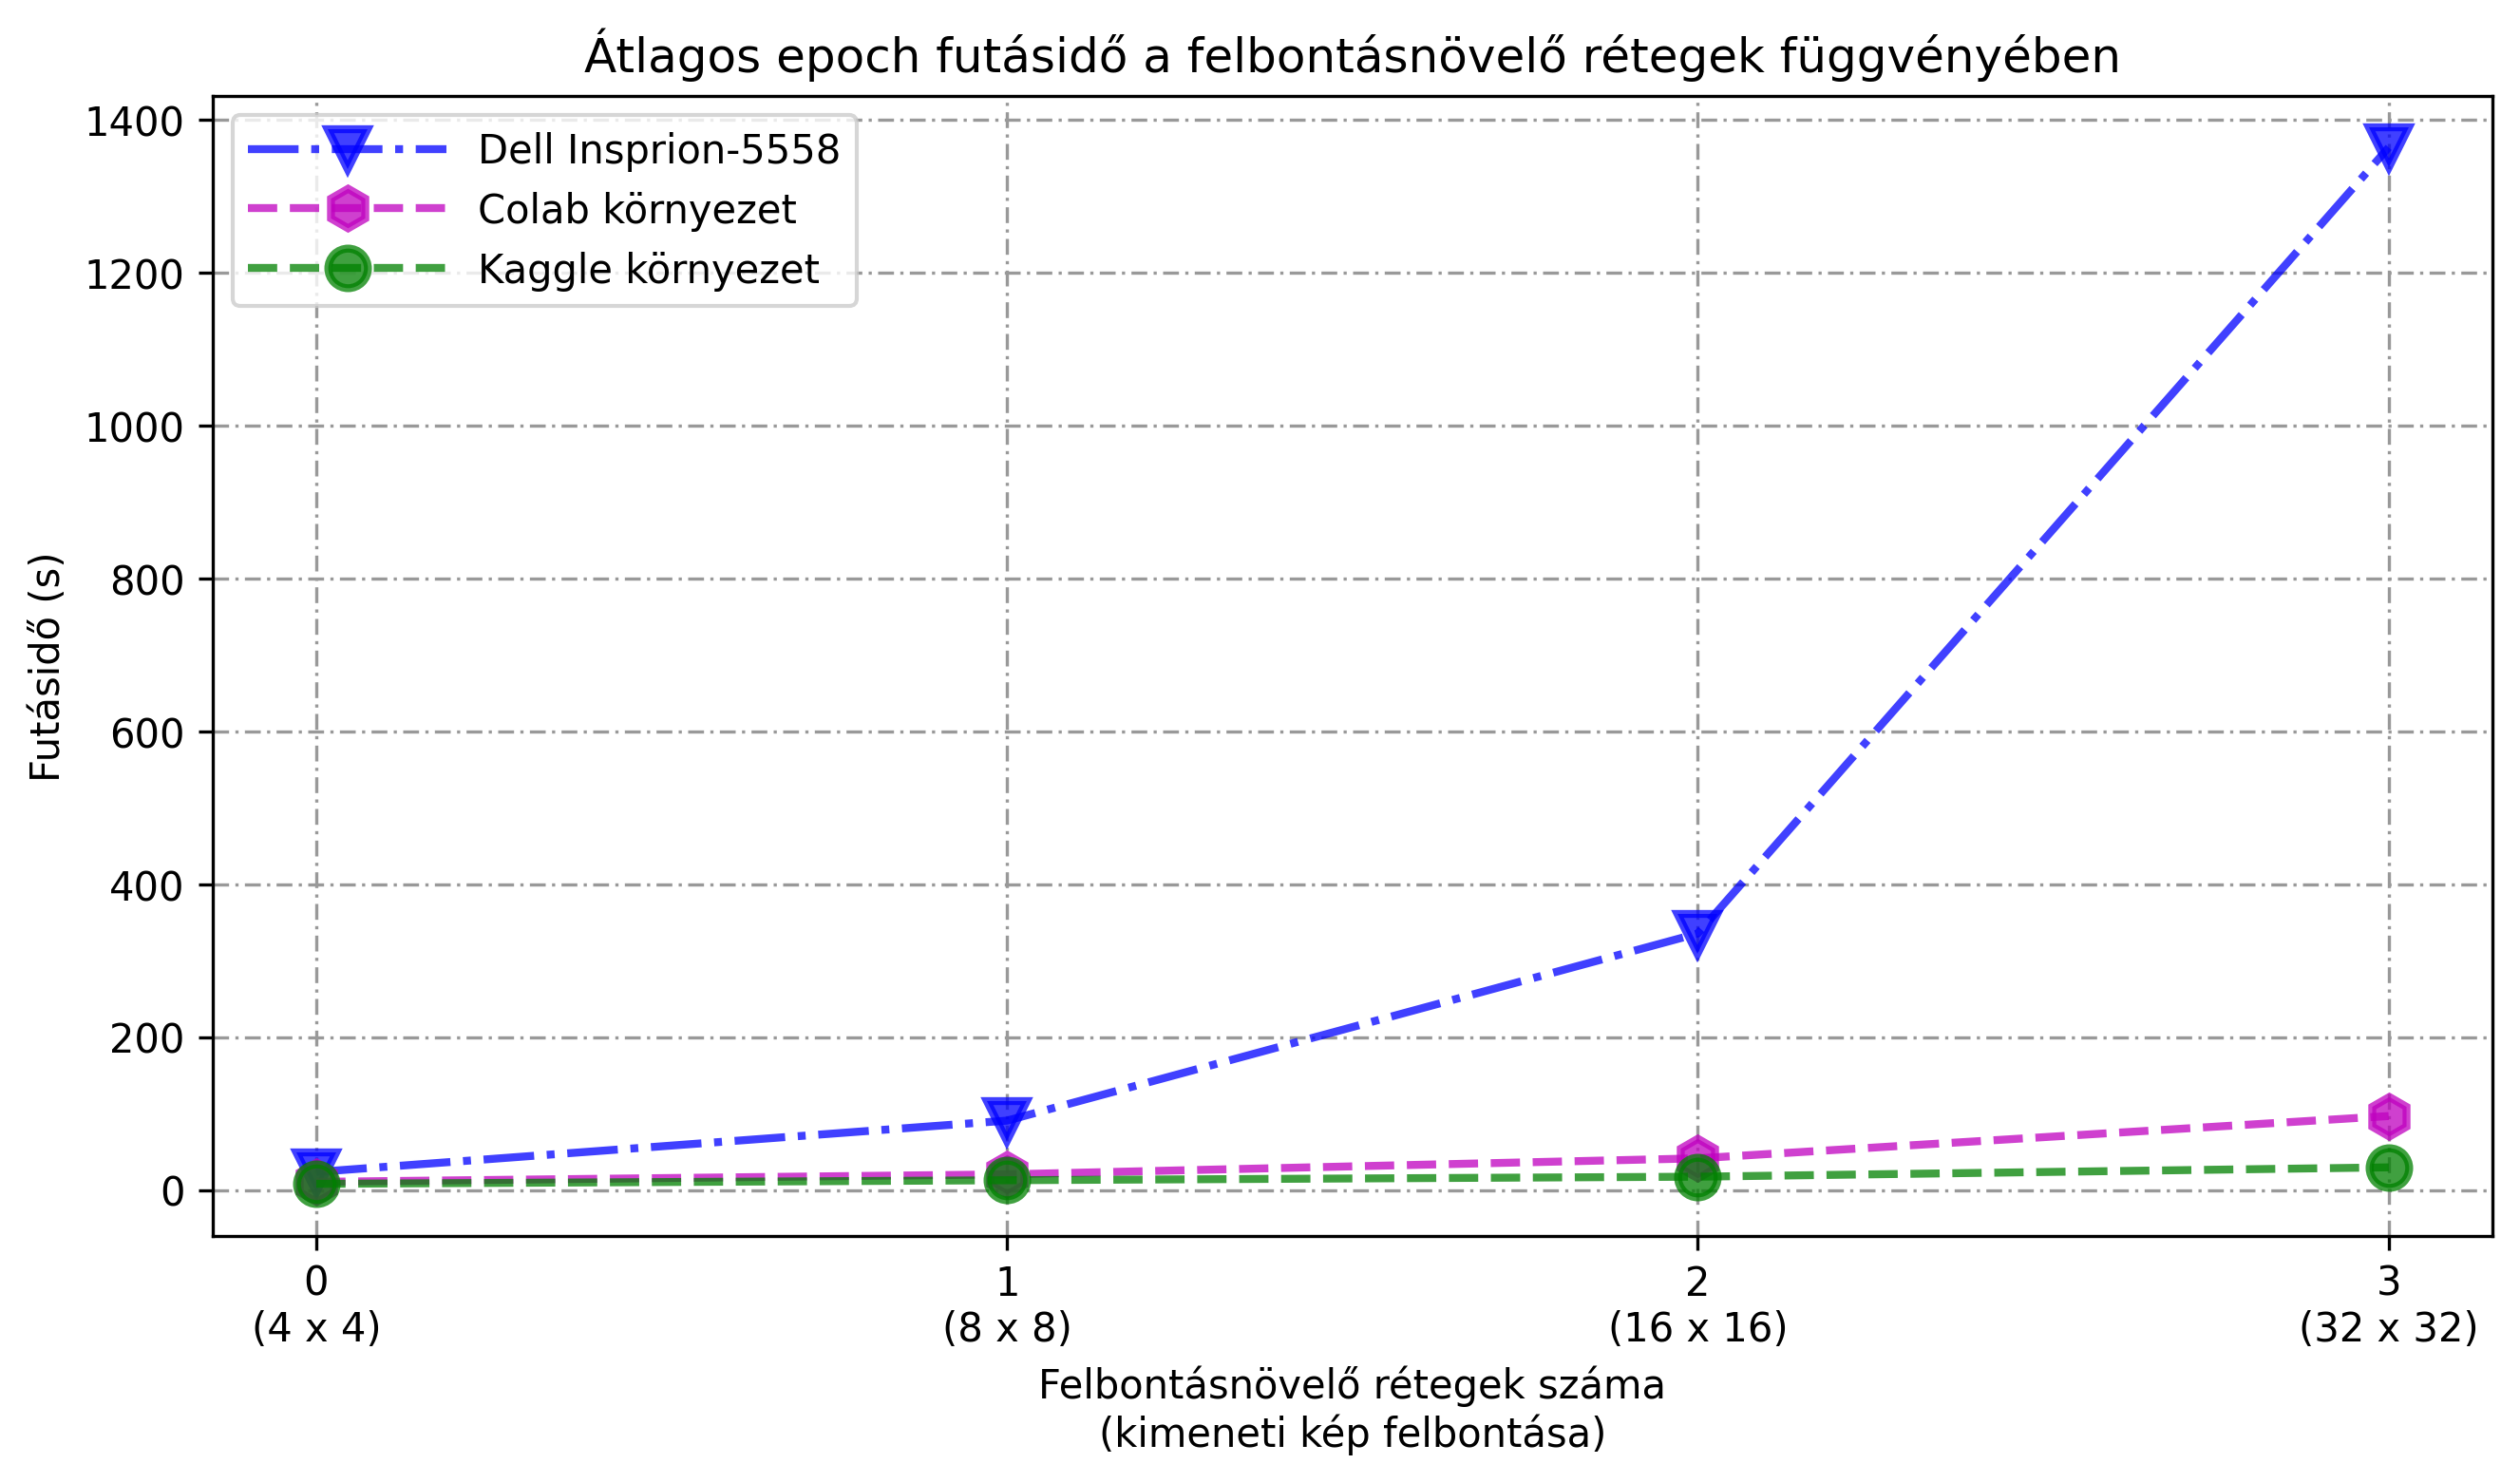
\includegraphics[width=15cm]{images/runtime.png}
\caption{Runtime ábra}
\label{fig:runtime}
\end{figure}

Mint látható, a laptopom igen alulmaradt a két virtuális környezettel szemben.


A dolgozat terjedelme (a mellékletek nélkül számítva) diplomamunka esetén 60-90, szakdolgozat esetén 40-60 oldal között optimális.

Az alábbi tagolás sorrendjének betartása nem kötelező, de az arányok lényegesek!
\begin{enumerate}
	\item Bevezető\\
Feladat ismertetése, honnan jött az ötlet, kitőzött célok, követelmények, elvárások. (~ 2 oldal)
	\item Irodalom feldolgozás, háttér információk (~ 10\%, de elméleti területen írt dolgozatok esetében ez akár 30\% is lehet)
	\begin{itemize}
		\item Ha cég megbízásából dolgozunk, ebben a részben lehet ismertetni a vállalatot. 
		\item Elméleti háttér ismertetése, hivatkozva a felhasznált irodalomra. 
	\end{itemize}
	\item A feladat megoldásához rendelkezésre álló technikák, technológiák, fejlesztőeszközök ismertetése, összehasonlítása, (előnyök, hátrányok ütköztetése, felhasználhatóság mérlegelése). (~ 25\%)
	\item Saját teljesítmény előállításához ténylegesen felhasznált eszközök részletes ismertetése; a kiválasztás szempontjai, telepítés, használatba vétel előfeltételei és lépései (ha azok nem magától értetődők). (~ 20\%)
	\item Saját munkánk (alkalmazásfejlesztés, mérés, tervezés stb.) részletes leírása, az eredmények szemléletes ismertetése. (~ 35\%)
	\item Összegzés\\ Tapasztalatok, eredmények összegzése; a feladat elkészítése során felmerült nehézségek, elkövetett hibák; jövőbeni fejlesztési lehetőségek. (~10\%)
\end{enumerate}